%\addtocontents{toc}{ \vspace{5mm} \hrule \par}

\chapter{Contenido adicional}\label{sec:apendice}

\section{Estructura del proyecto}\label{ap:estructura}
La estructura escogida para el proyecto ha sido la marcada por el ``Makefile'' proporcionado por el \textit{toolchain} utilizado. La estructura es la observada en la Figura~\ref{fig:ap_estructura}.

\begin{figure}[h]
	\centering
	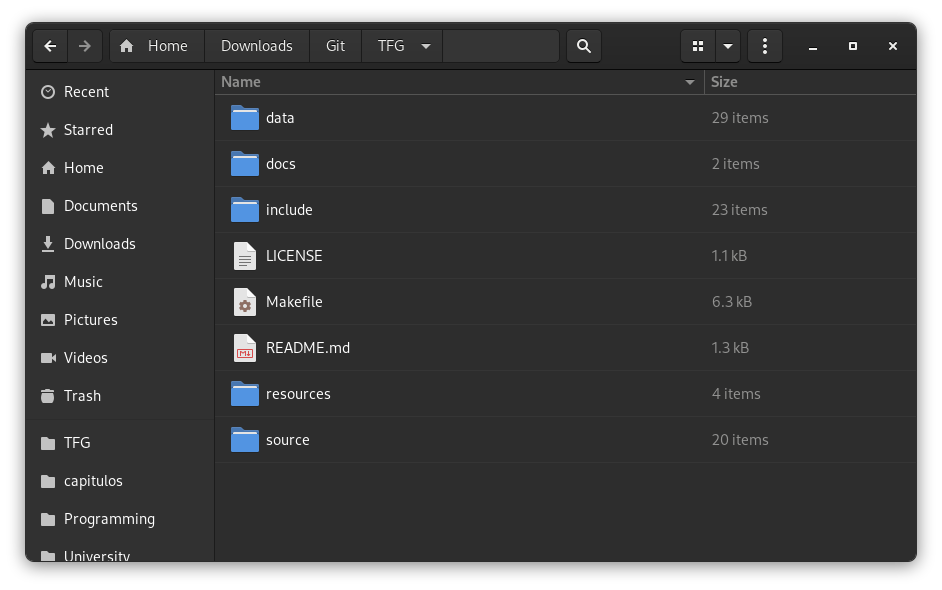
\includegraphics[width=.7\textwidth]{capitulos/apendice/estructura.png}
	\caption{Estructura del proyecto.}\label{fig:ap_estructura}
\end{figure}
\FloatBarrier{}

Cada uno de los archivos y directorios mostrados tiene la siguiente función:

\begin{itemize}
	\item data: En esta carpeta se localizan todos los archivos binarios, como imágenes y pistas de audio, que posteriormente son convertidas a un formato compatible con la consola.
	\item docs: Aquí reside el documento \LaTeX~junto con otros apuntes en sucio realizados durante el desarrollo del juego.
	\item include: Todas las cabeceras del código residen aquí.
	\item LICENSE: En este archivo se describen las condiciones de la licencia escogida, la MIT\footnote{https://opensource.org/licenses/MIT}.
	\item Makefile: El archivo que permite a ``make'' compilar el código y convertir los \textit{assets} del juego. Precisa una instalación previa de \textit{devkitpro} dado que utiliza varias herramientas incluidas en el \textit{toolchain}.
	\item README.md: En este archivo se incluyen varias instrucciones a los usuarios que visitan el repositorio GitHub.
	\item resources: En esta carpeta se incluyen varios recursos y documentación. Puede servir de utilidad para en caso de perder acceso a la red.
	\item source: Aquí reside todo el código del juego.
\end{itemize}

\section{Personajes}\label{ap:personajes}

\begin{figure}[h]
	\centering
	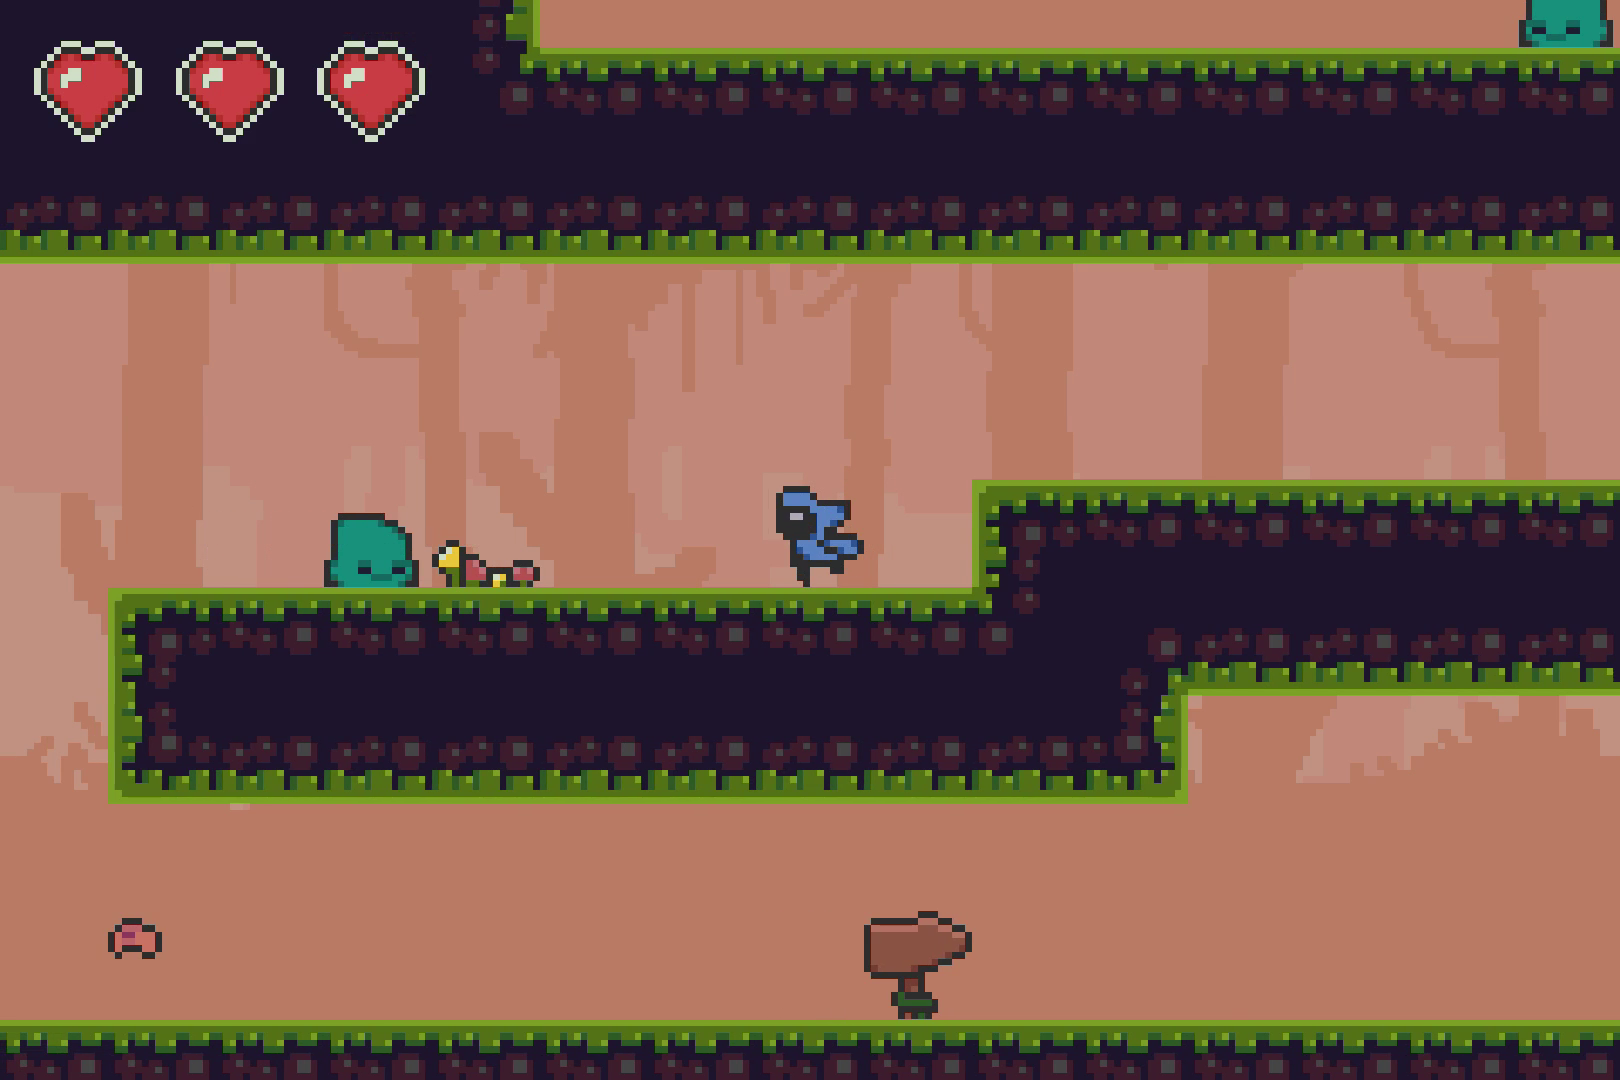
\includegraphics[width=.6\textwidth]{capitulos/apendice/sprites_1.png}
	\caption{Variante azul corriendo.}\label{fig:ap_sprites_1}
\end{figure}

\begin{figure}[h]
	\centering
	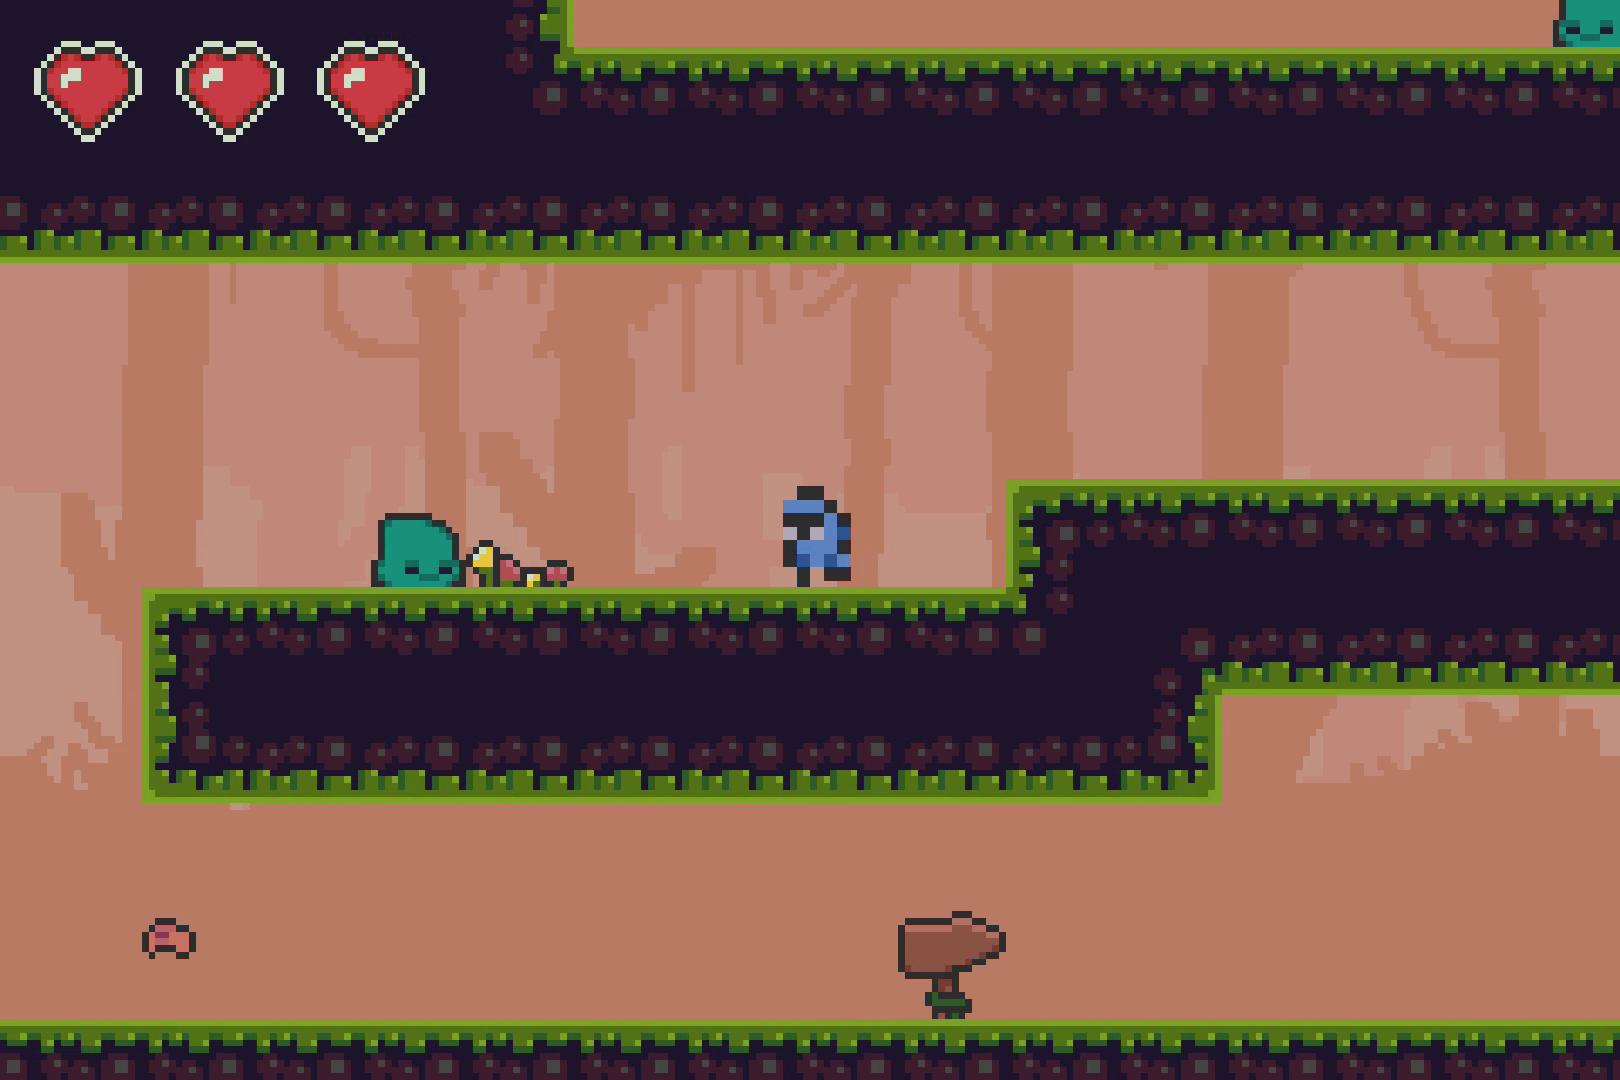
\includegraphics[width=.6\textwidth]{capitulos/apendice/sprites_2.png}
	\caption{Variante azul iniciando la transformación.}\label{fig:ap_sprites_2}
\end{figure}

\begin{figure}[h]
	\centering
	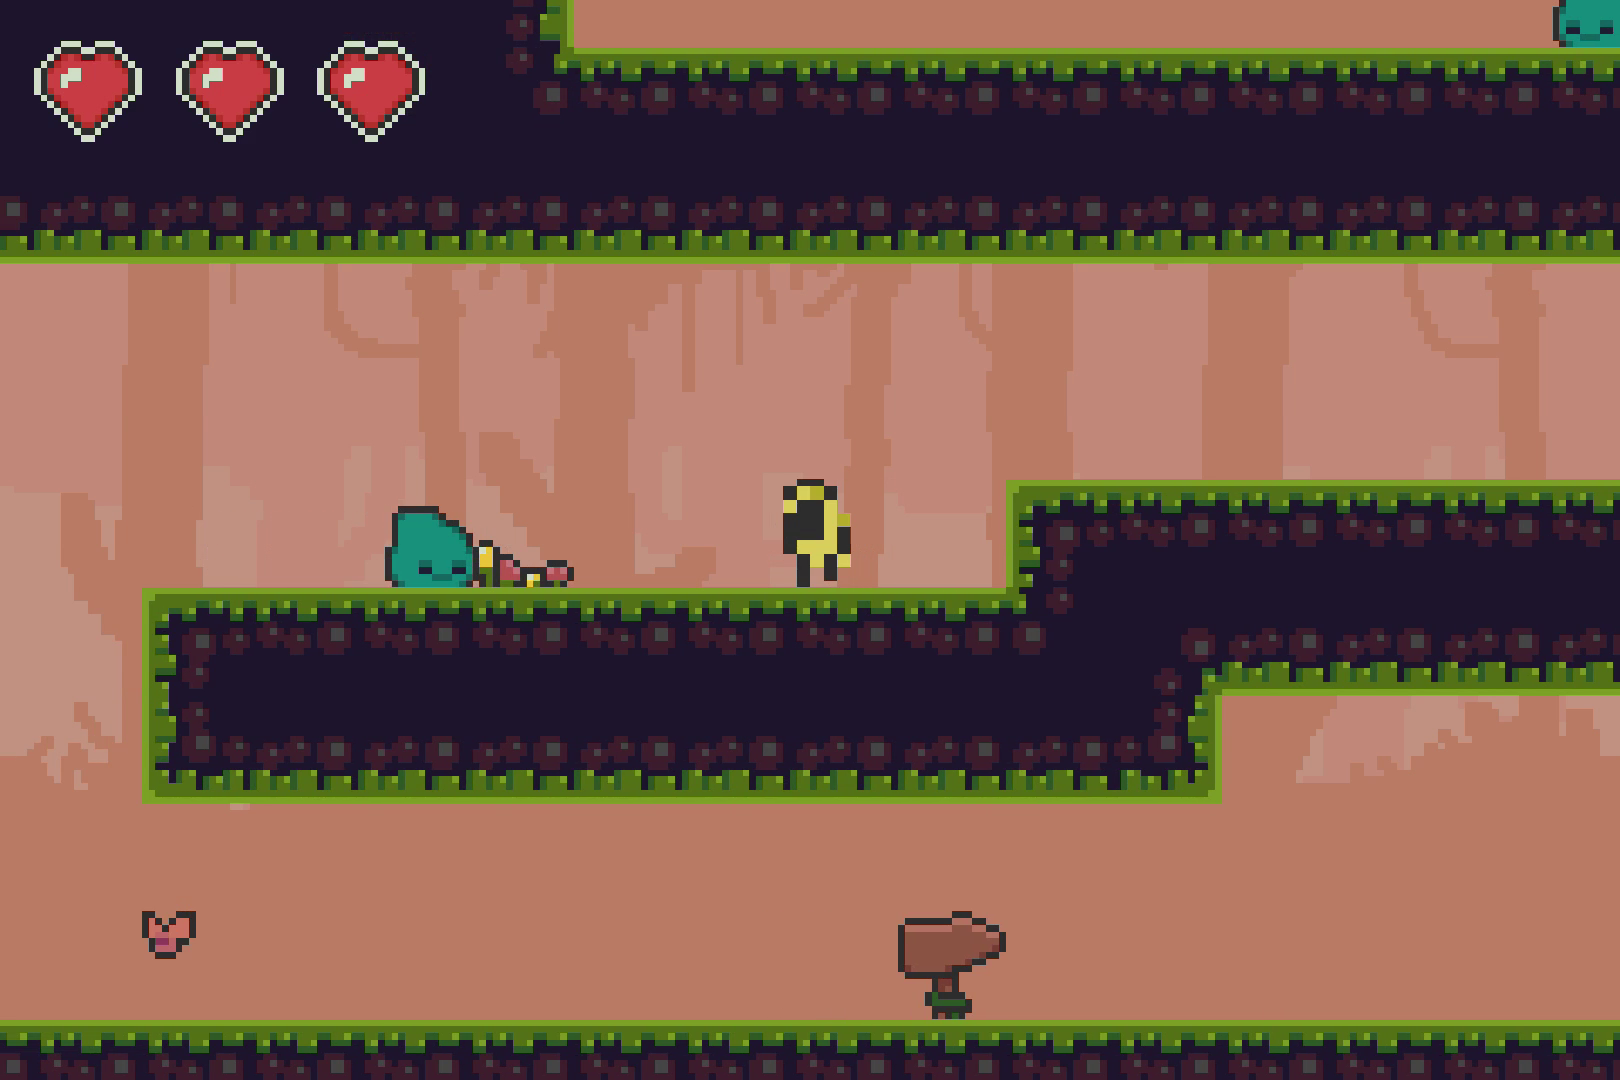
\includegraphics[width=.6\textwidth]{capitulos/apendice/sprites_3.png}
	\caption{Últimos fotogramas de la transformación de la variante azul a la dorada.}\label{fig:ap_sprites_3}
\end{figure}

\begin{figure}[h]
	\centering
	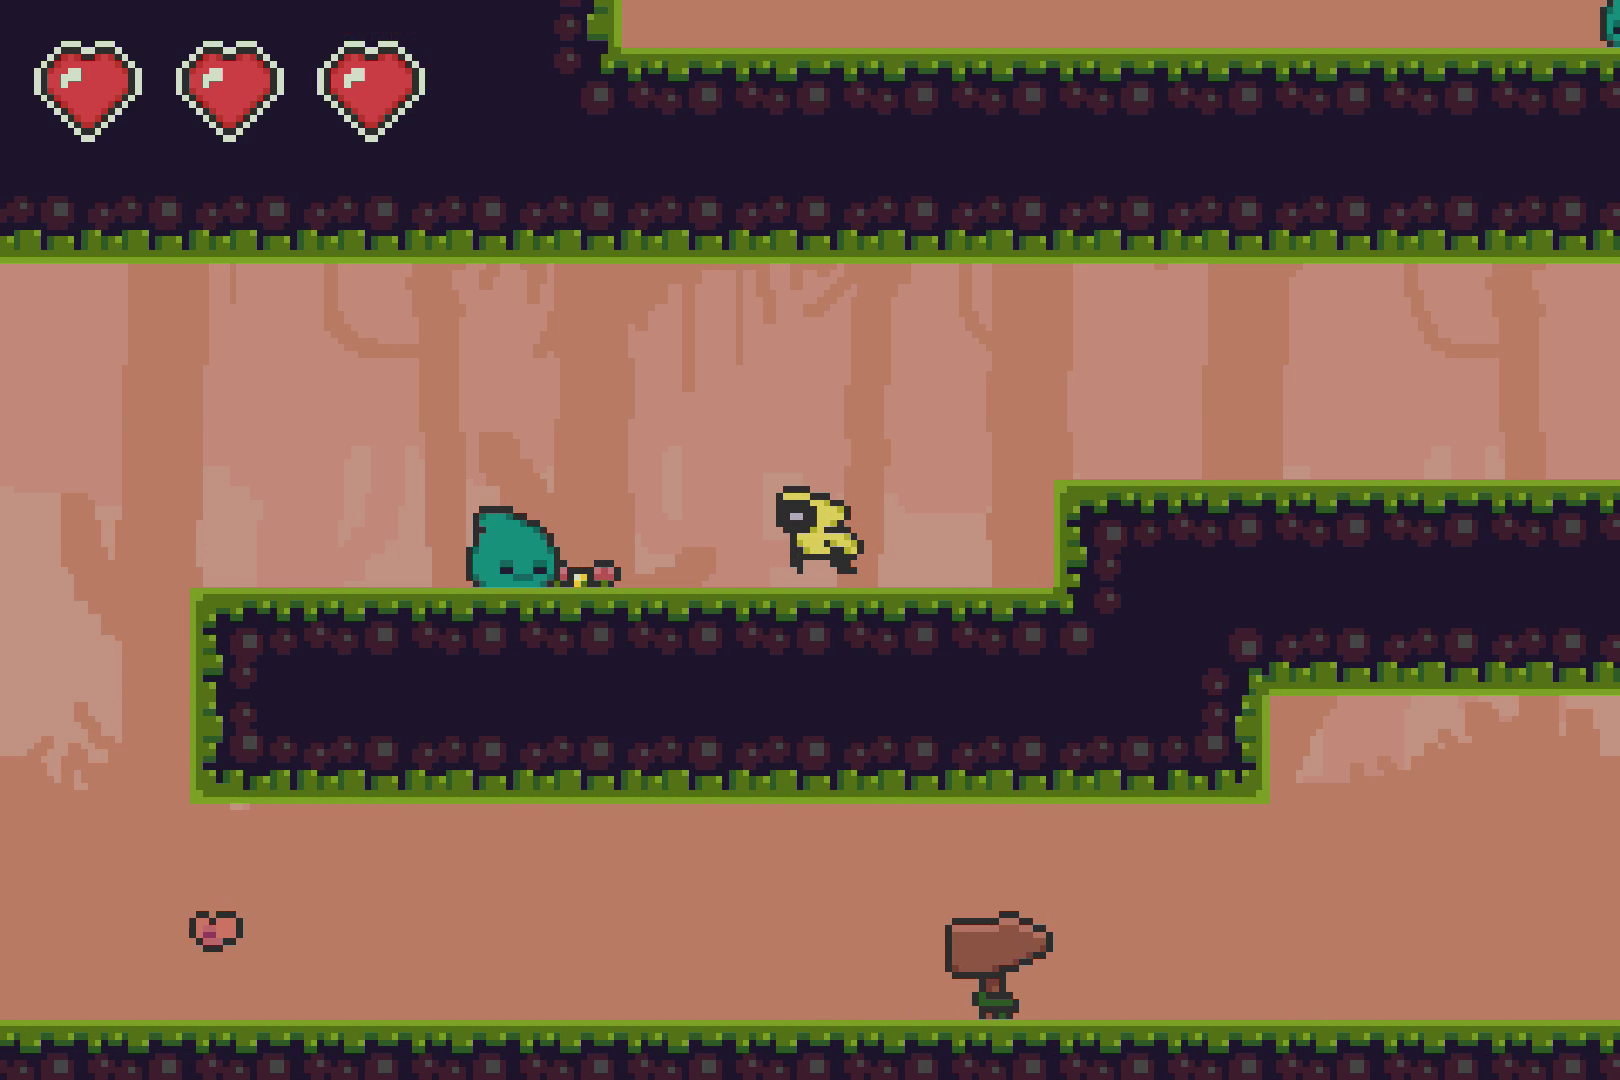
\includegraphics[width=.6\textwidth]{capitulos/apendice/sprites_4.png}
	\caption{Variante dorada.}\label{fig:ap_sprites_4}
\end{figure}

\begin{figure}[h]
	\centering
	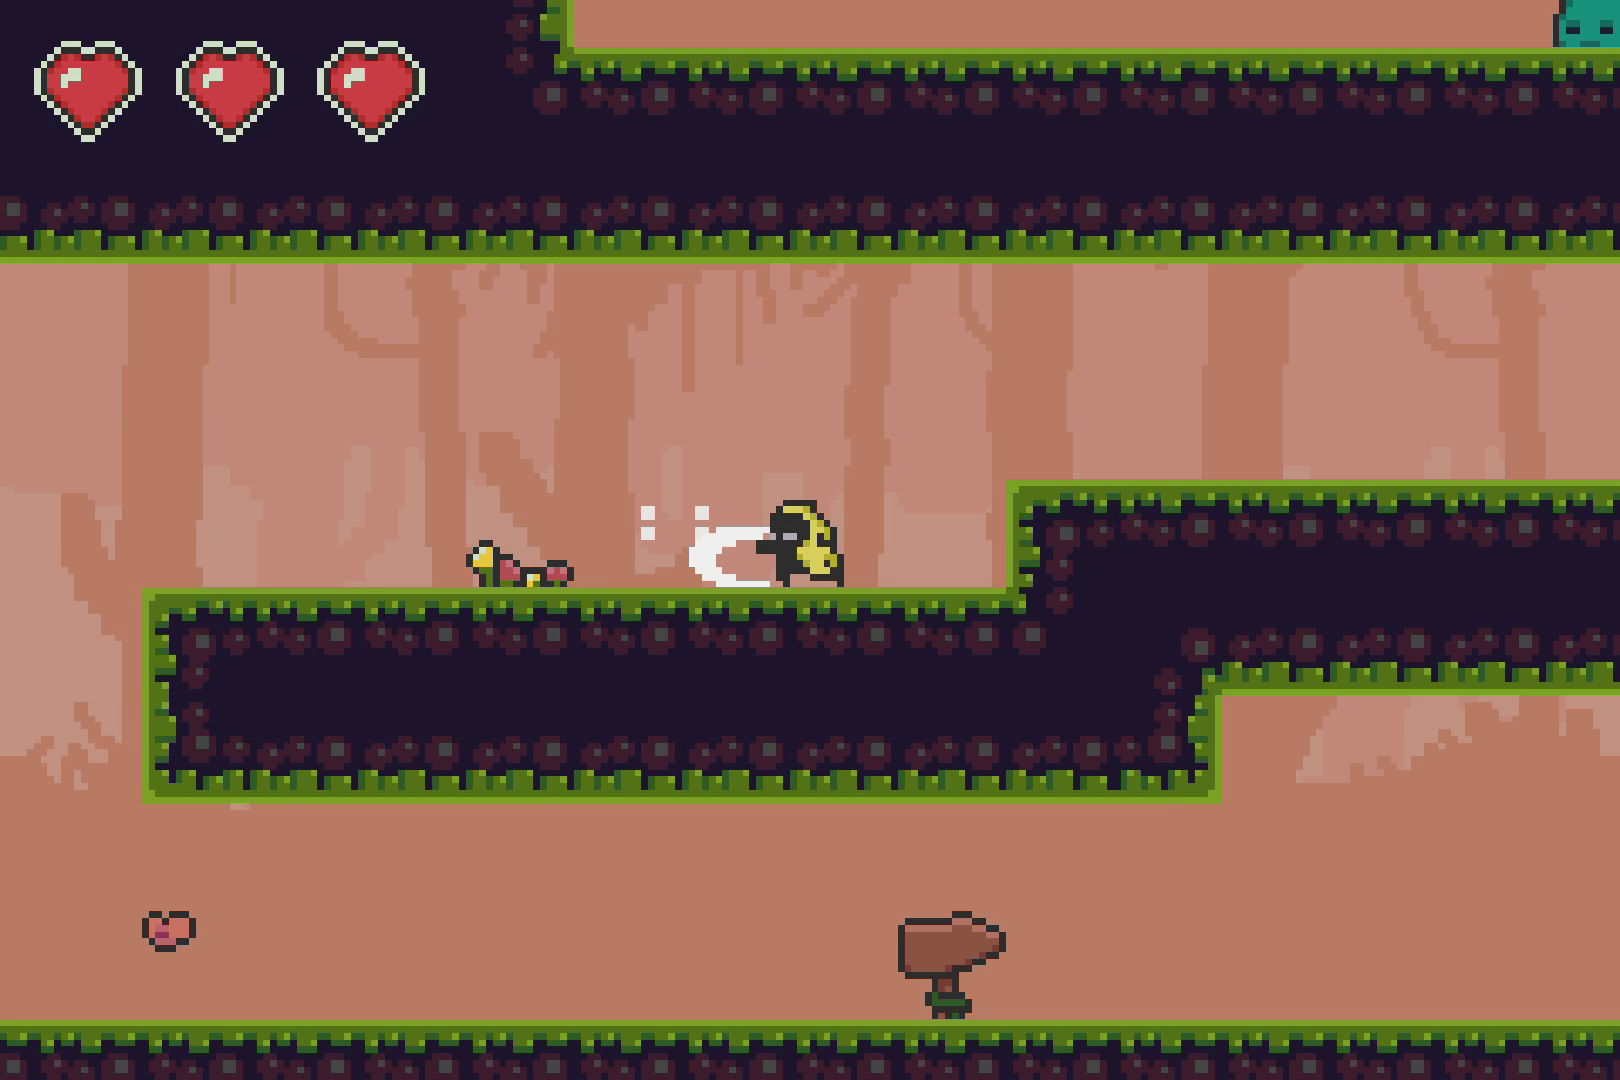
\includegraphics[width=.6\textwidth]{capitulos/apendice/sprites_5.png}
	\caption{Ataque del personaje principal. además se observa la muerte del ``monstruo verde''.}\label{fig:ap_sprites_5}
\end{figure}

\begin{figure}[h]
	\centering
	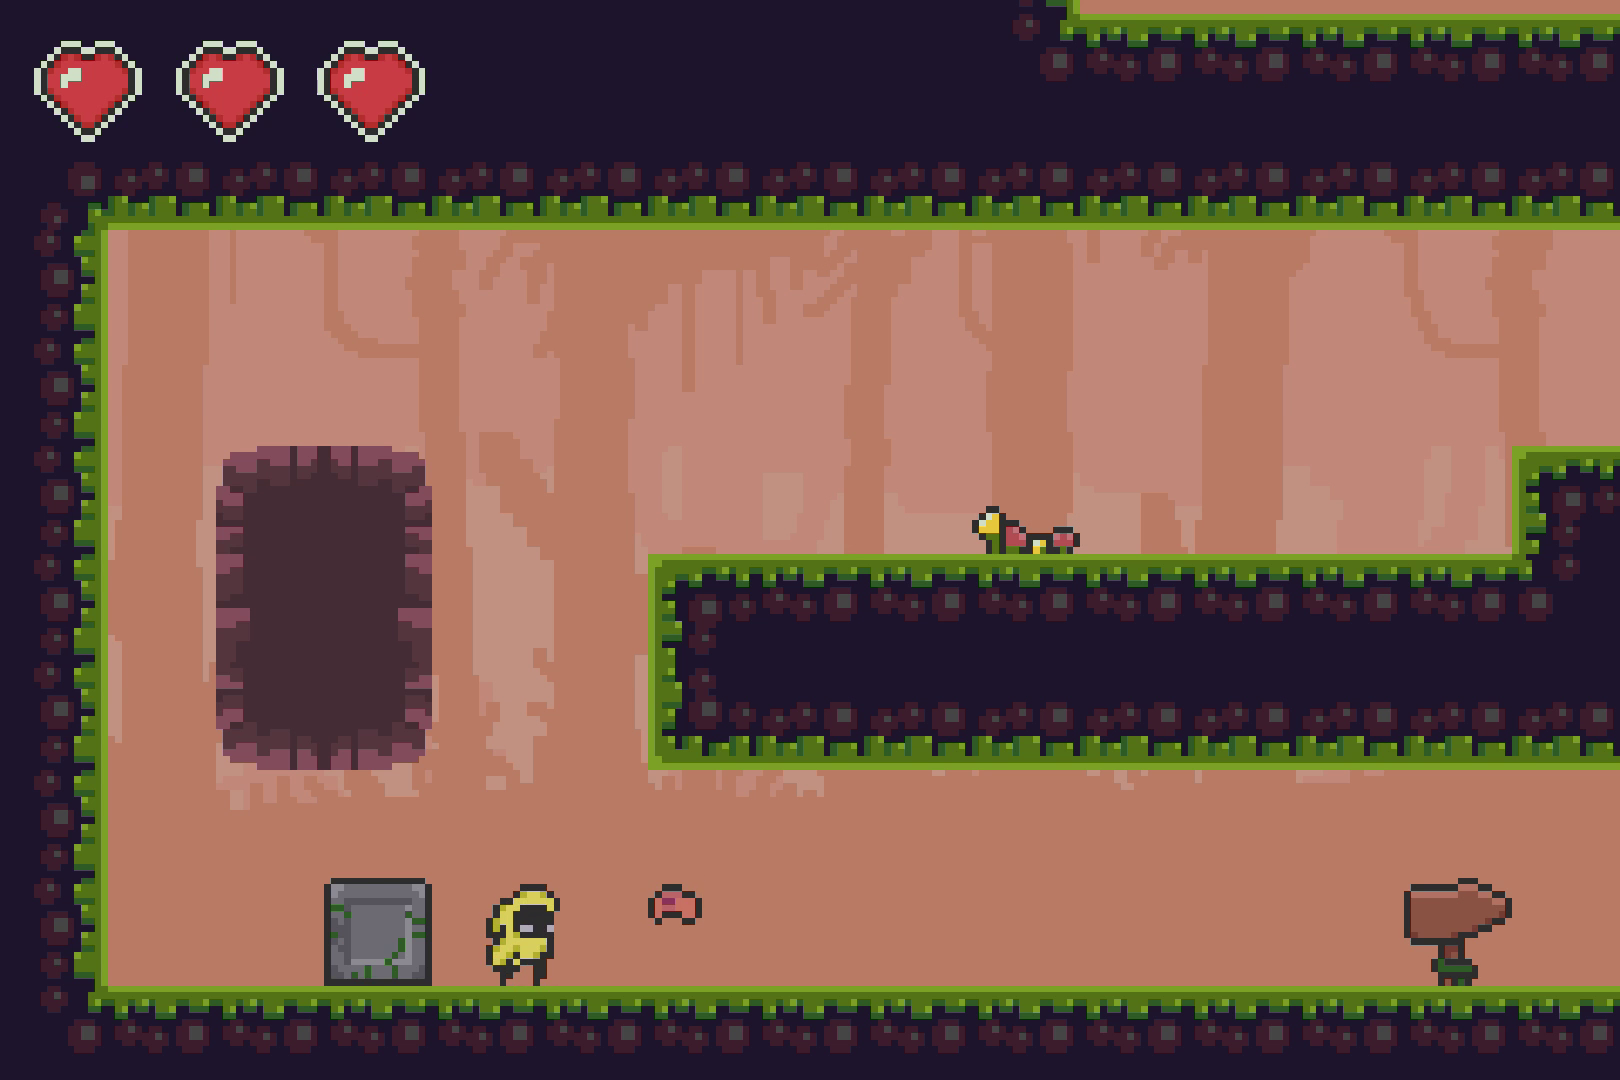
\includegraphics[width=.6\textwidth]{capitulos/apendice/sprites_7.png}
	\caption{Variante dorada del personaje principal junto a uno de los enemigos.}\label{fig:ap_sprites_7}
\end{figure}

\begin{figure}[h]
	\centering
	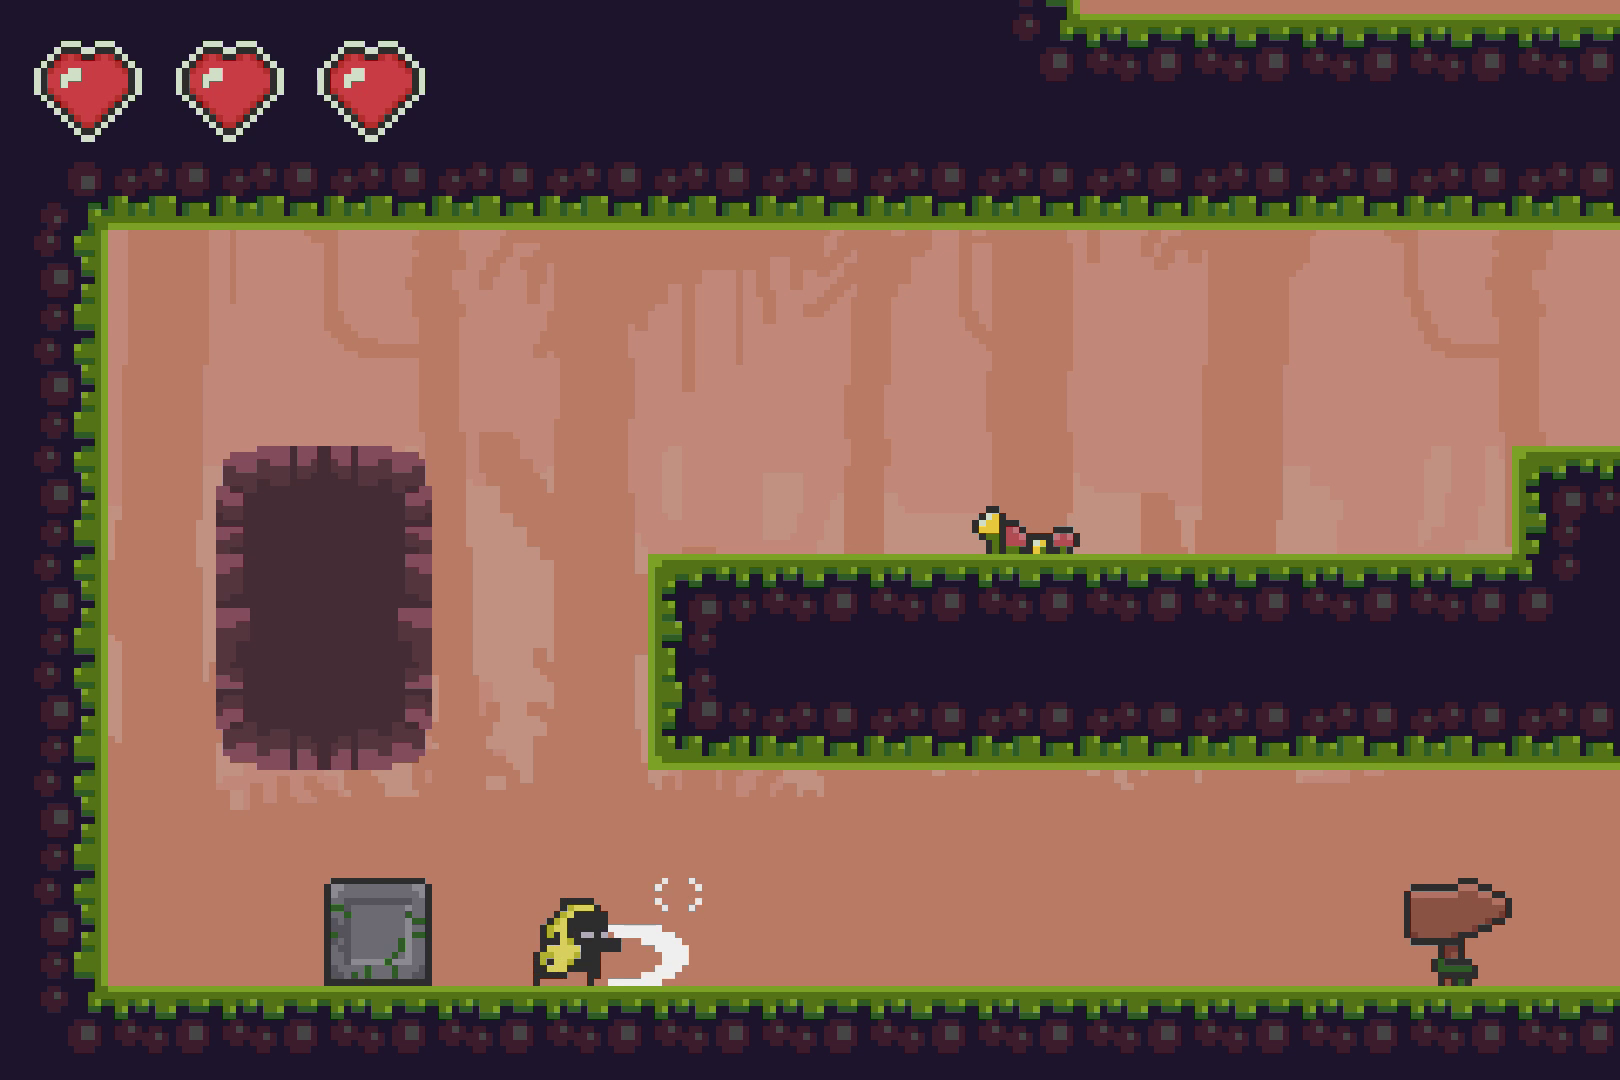
\includegraphics[width=.6\textwidth]{capitulos/apendice/sprites_6.png}
	\caption{Ataque del personaje principal. Además se observa la muerte de la ``mosca''.}\label{fig:ap_sprites_6}
\end{figure}

\begin{figure}[h]
	\centering
	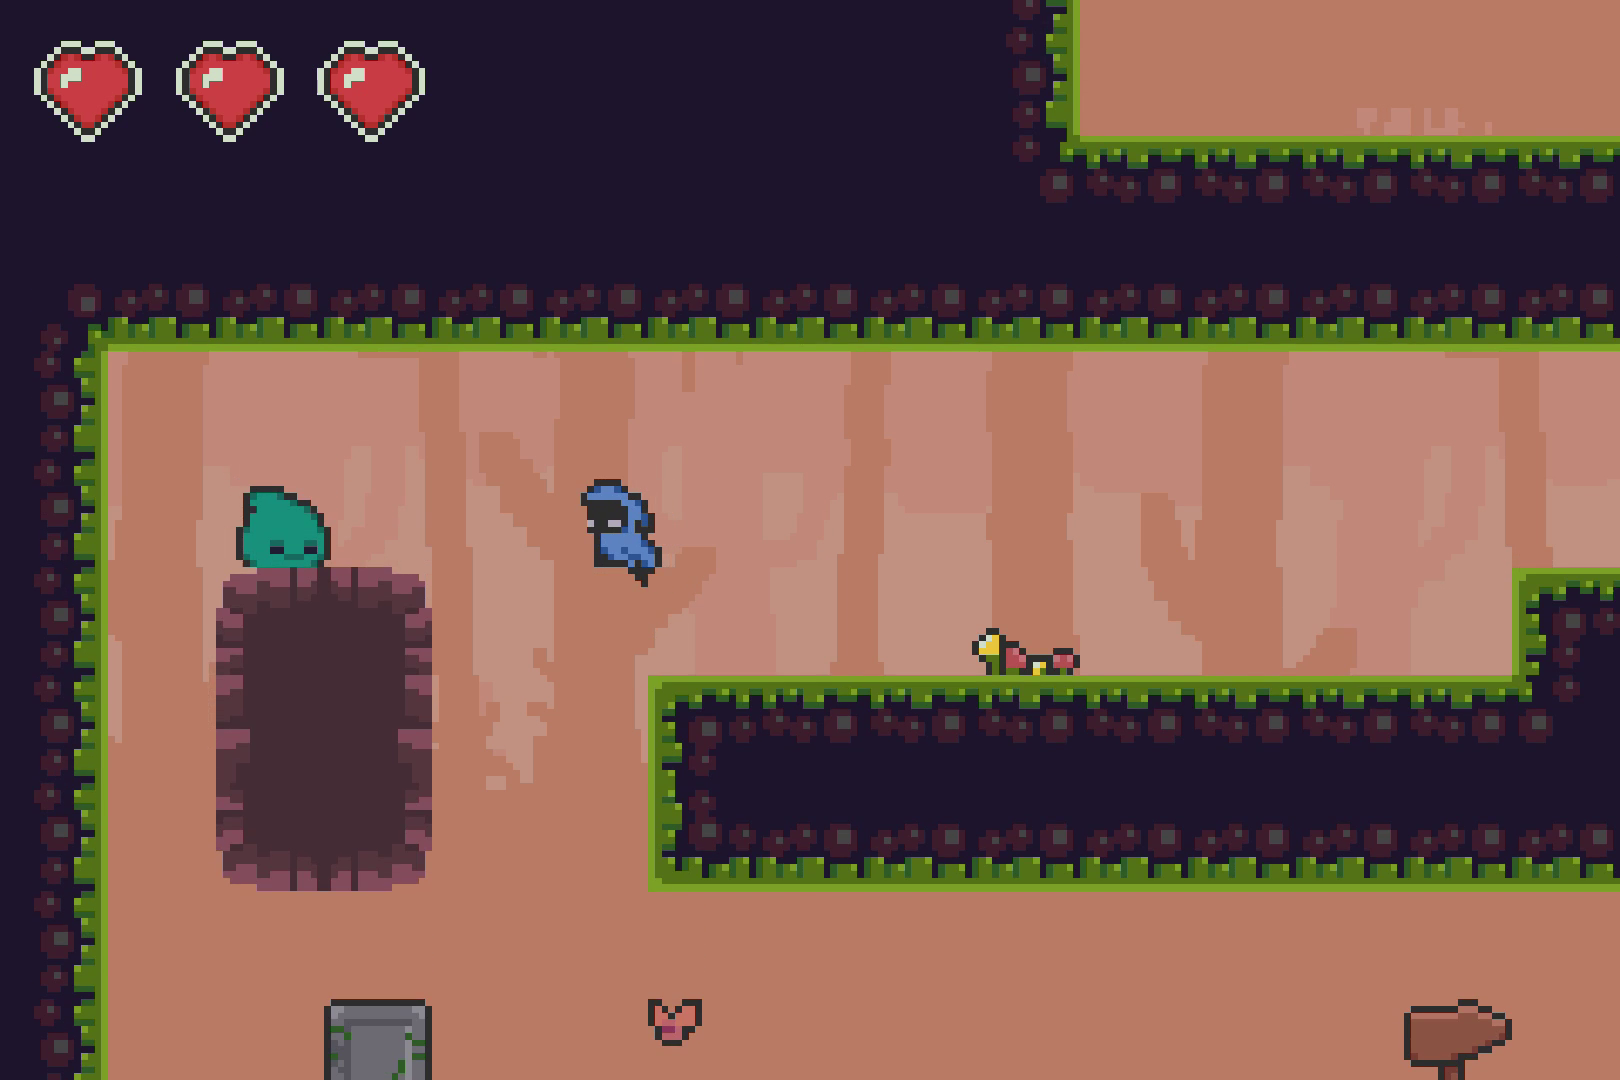
\includegraphics[width=.6\textwidth]{capitulos/apendice/sprites_8.png}
	\caption{El personaje principal saltando.}\label{fig:ap_sprites_8}
\end{figure}

\begin{figure}[h]
	\centering
	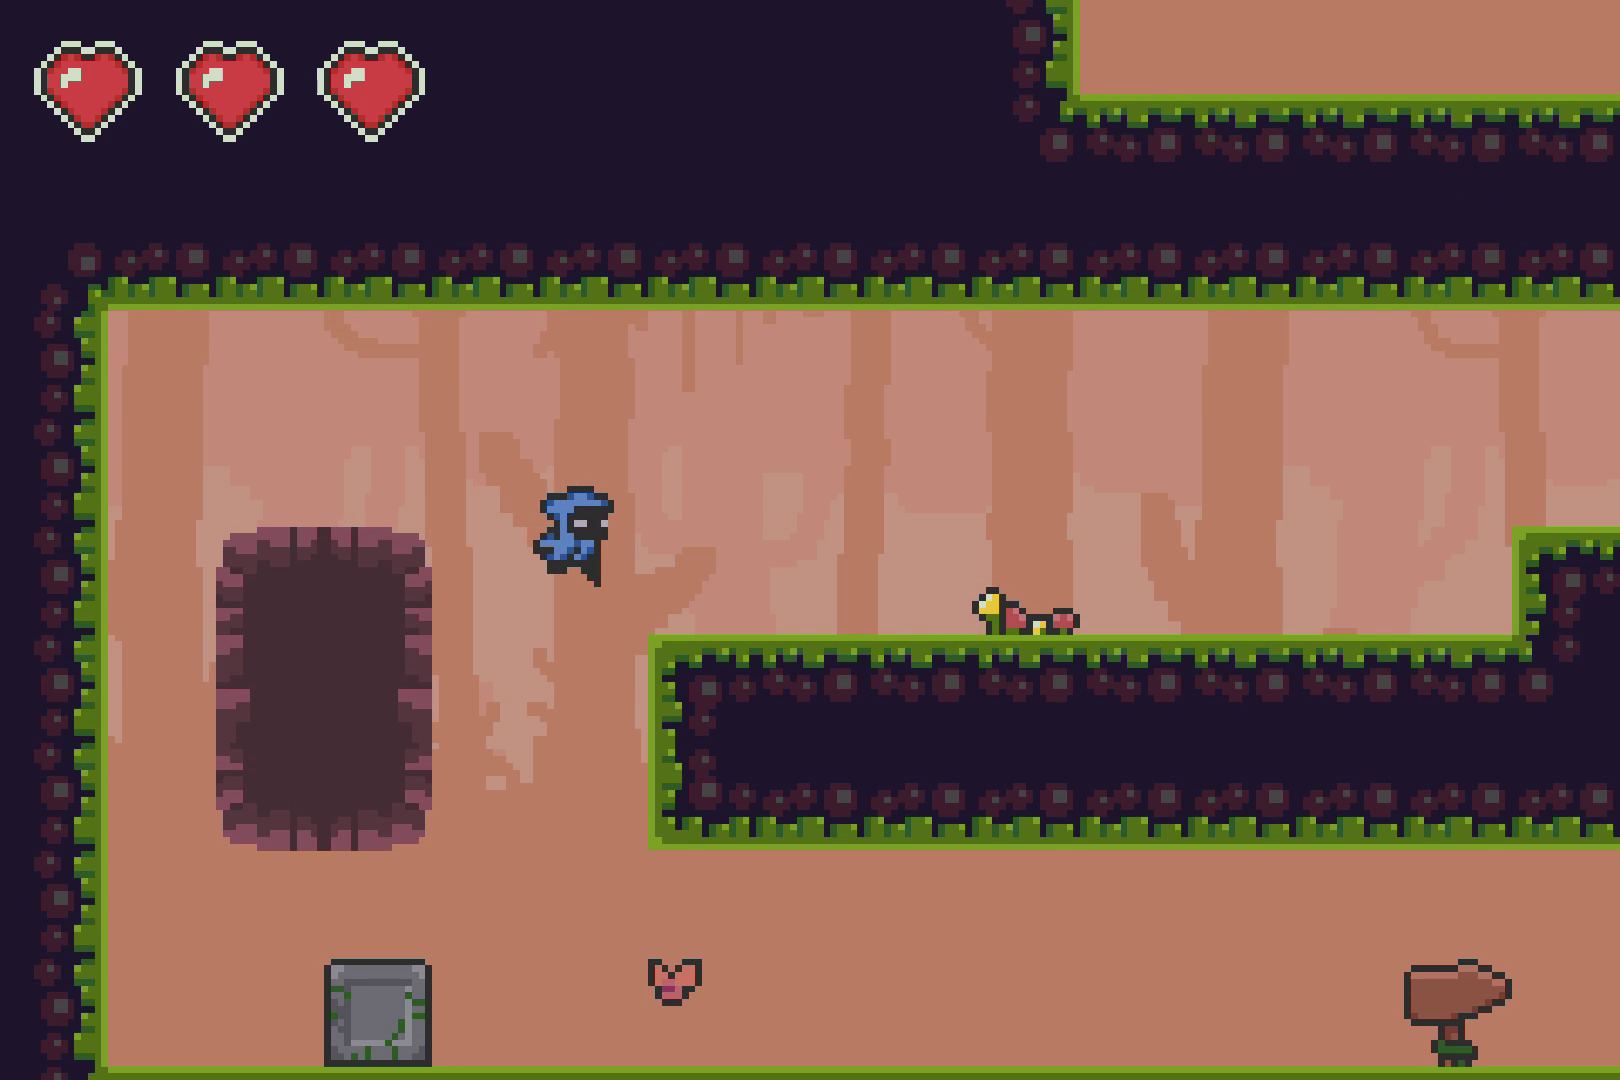
\includegraphics[width=.6\textwidth]{capitulos/apendice/sprites_9.png}
	\caption{El personaje principal cayendo.}\label{fig:ap_sprites_9}
\end{figure}

\begin{figure}[h]
	\centering
	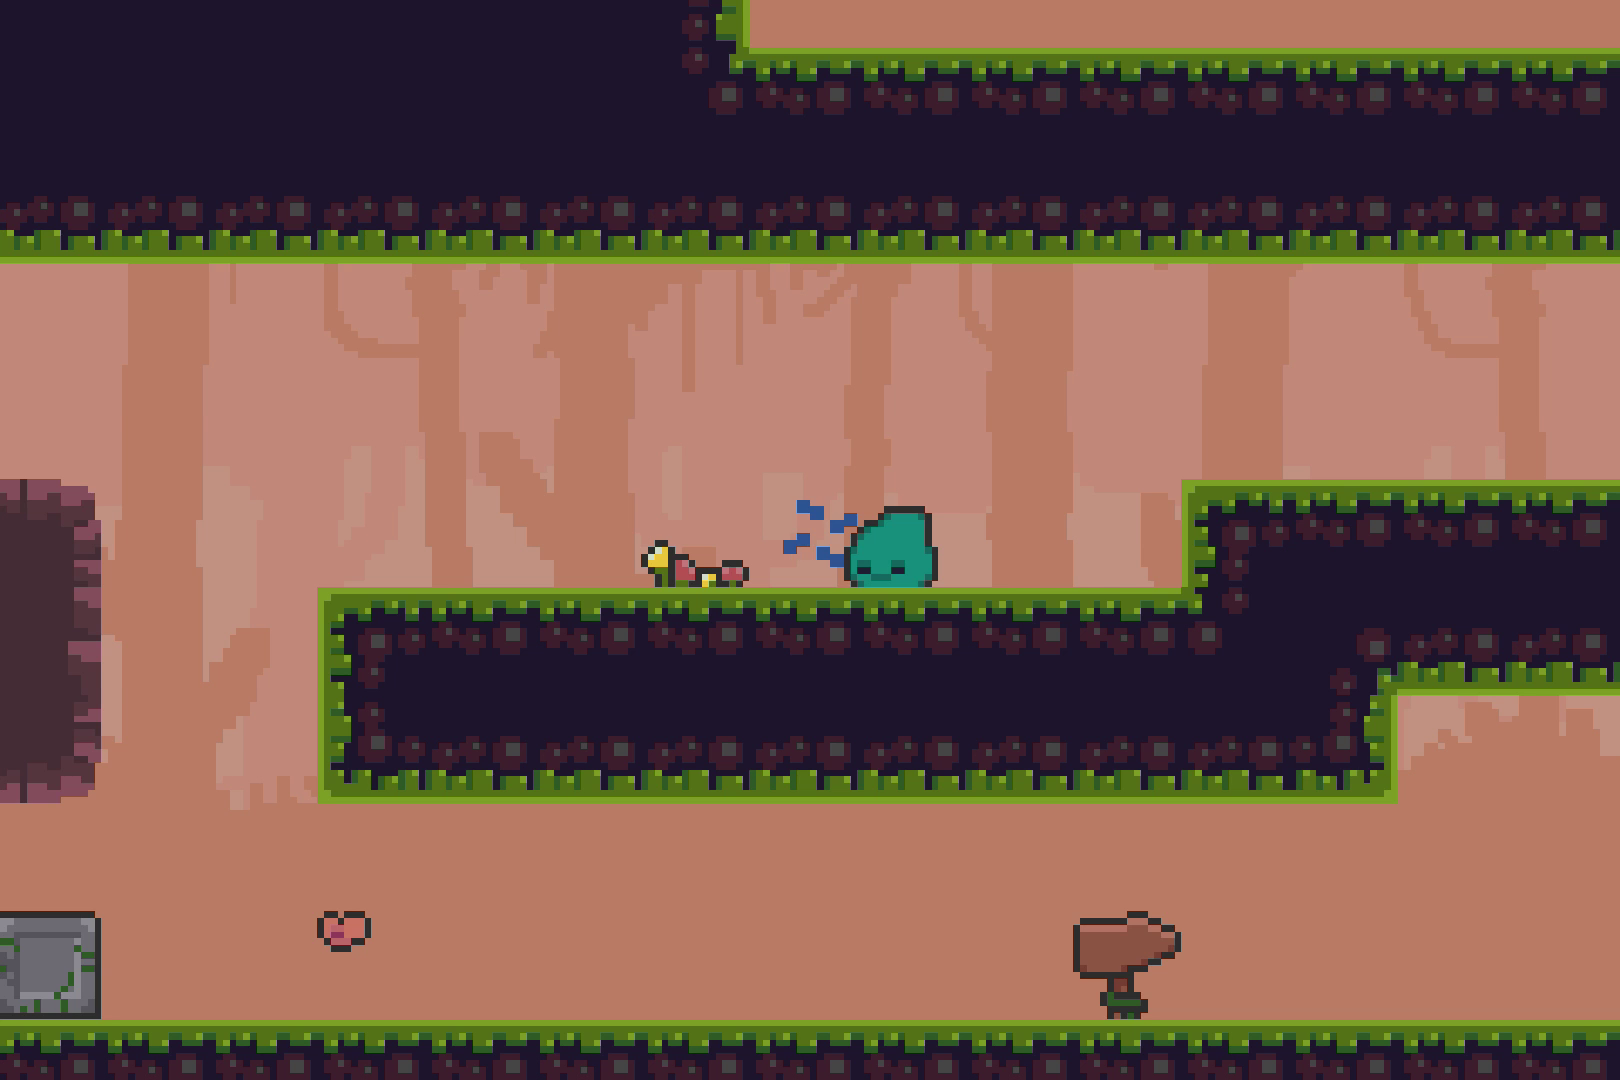
\includegraphics[width=.6\textwidth]{capitulos/apendice/sprites_10.png}
	\caption{El personaje principal desapareciendo al no tener vida.}\label{fig:ap_sprites_10}
\end{figure}
\FloatBarrier{}


\section{Registros}\label{ap:registros}

\begin{figure}[h]
	\centering
	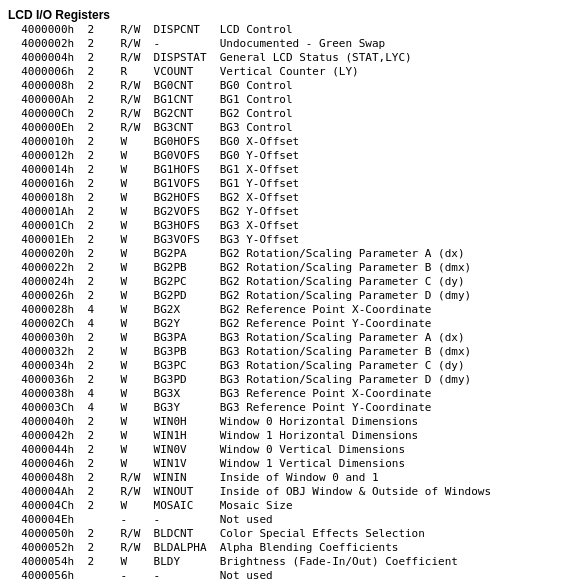
\includegraphics[width=.9\textwidth]{capitulos/apendice/reg_1.png}
	\caption{Registros LCD.}\label{fig:ap_reg_1}
\end{figure}

\begin{figure}[h]
	\centering
	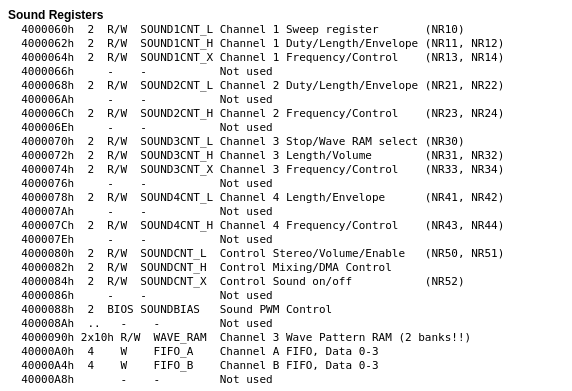
\includegraphics[width=.9\textwidth]{capitulos/apendice/reg_2.png}
	\caption{Registros de Sonido.}\label{fig:ap_reg_2}
\end{figure}

\begin{figure}[h]
	\centering
	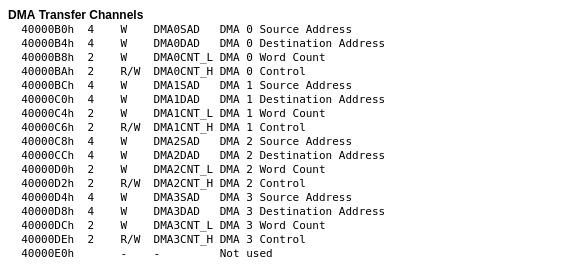
\includegraphics[width=.9\textwidth]{capitulos/apendice/reg_3.png}
	\caption{Registros \textit{Direct Memory Access}.}\label{fig:ap_reg_3}
\end{figure}

\begin{figure}[h]
	\centering
	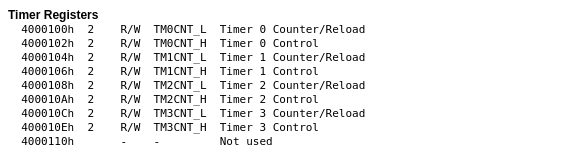
\includegraphics[width=.9\textwidth]{capitulos/apendice/reg_4.png}
	\caption{Registros de Temporización.}\label{fig:ap_reg_4}
\end{figure}

\begin{figure}[h]
	\centering
	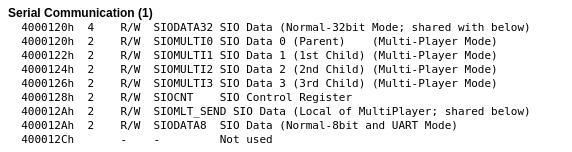
\includegraphics[width=.9\textwidth]{capitulos/apendice/reg_5.png}
	\caption{Registros de Comunicación Serial (1).}\label{fig:ap_reg_5}
\end{figure}

\begin{figure}[h]
	\centering
	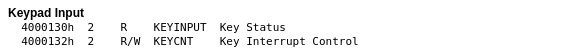
\includegraphics[width=.9\textwidth]{capitulos/apendice/reg_6.png}
	\caption{Registros de los botones.}\label{fig:ap_reg_6}
\end{figure}

\begin{figure}[h]
	\centering
	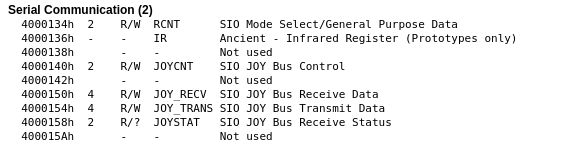
\includegraphics[width=.9\textwidth]{capitulos/apendice/reg_7.png}
	\caption{Registros de Comunicación Serial (2).}\label{fig:ap_reg_7}
\end{figure}

\begin{figure}[h]
	\centering
	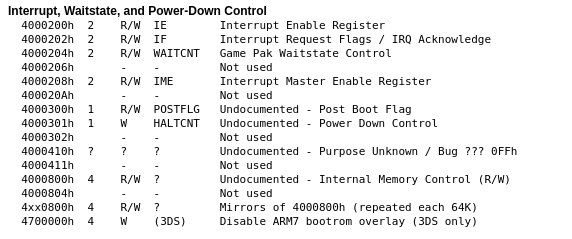
\includegraphics[width=.9\textwidth]{capitulos/apendice/reg_8.png}
	\caption{Registros de Interrupciones.}\label{fig:ap_reg_8}
\end{figure}
\FloatBarrier{}


\section{Escenas}\label{ap:escenas}

\begin{figure}[h]
	\centering
	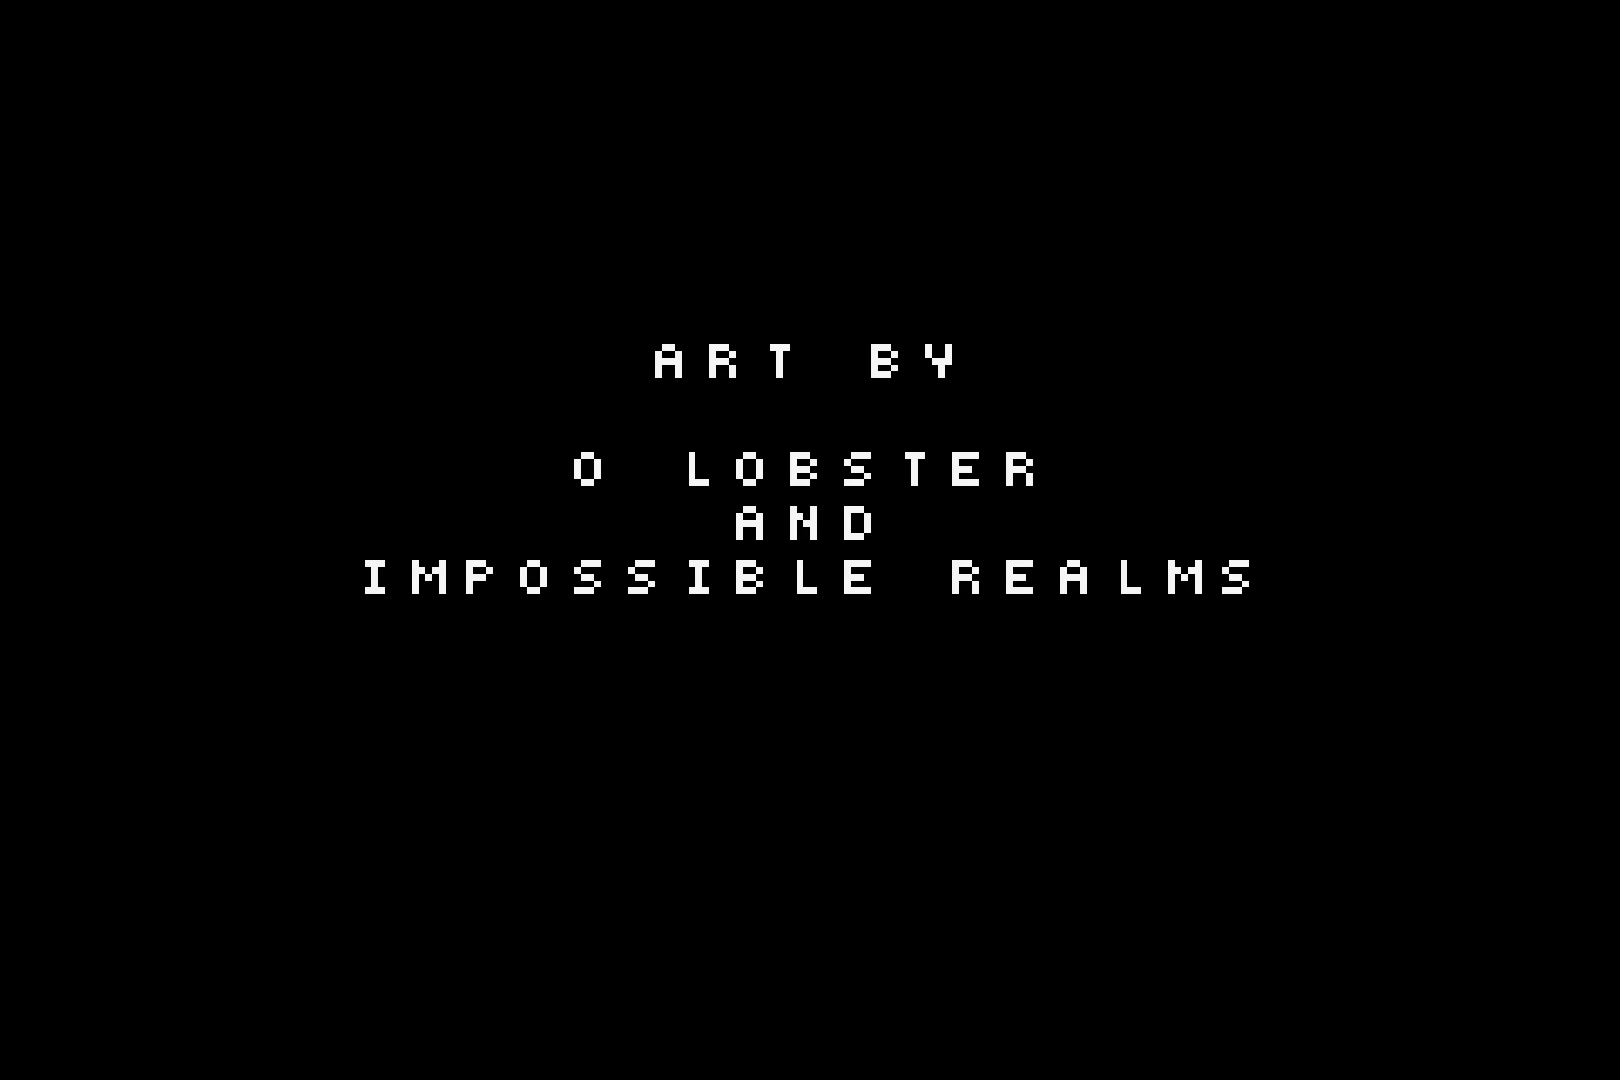
\includegraphics[height=6cm]{capitulos/apendice/credits_0.png}
	\caption{Créditos iniciales (1).}\label{fig:ap_credits_0}
\end{figure}

\vspace{3cm}

\begin{figure}[h]
	\centering
	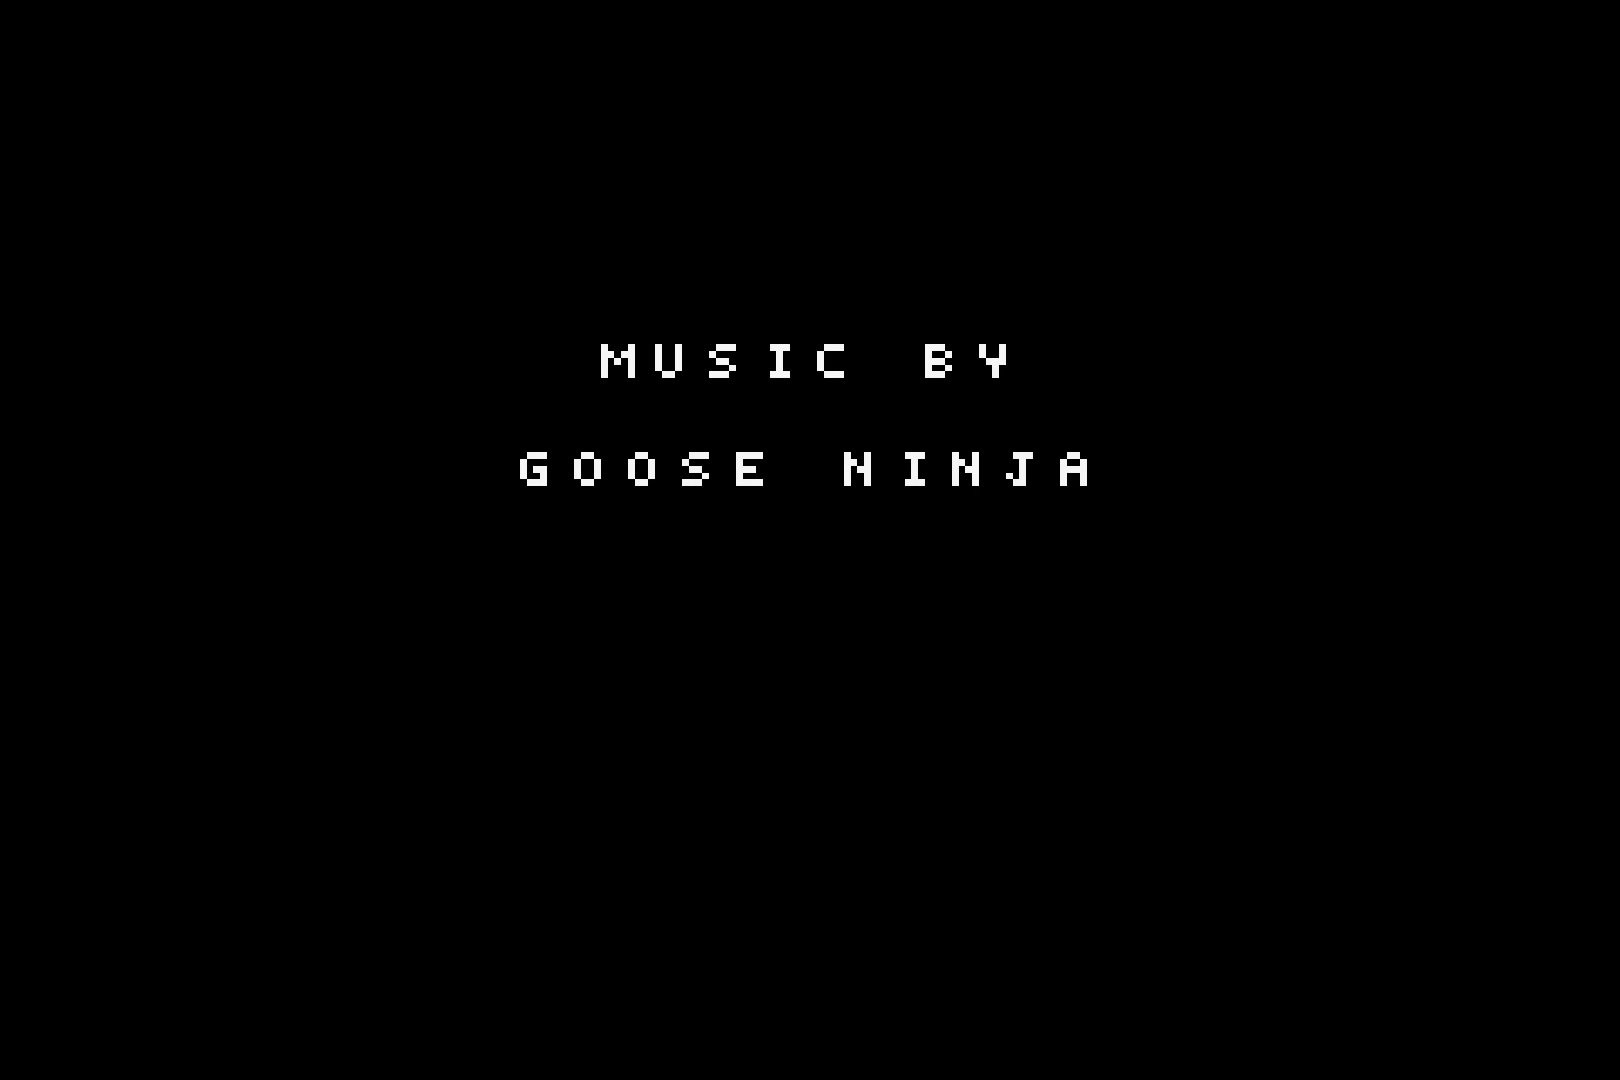
\includegraphics[height=6cm]{capitulos/apendice/credits_1.png}
	\caption{Créditos iniciales (2).}\label{fig:ap_credits_1}
\end{figure}

\begin{figure}[h]
	\centering
	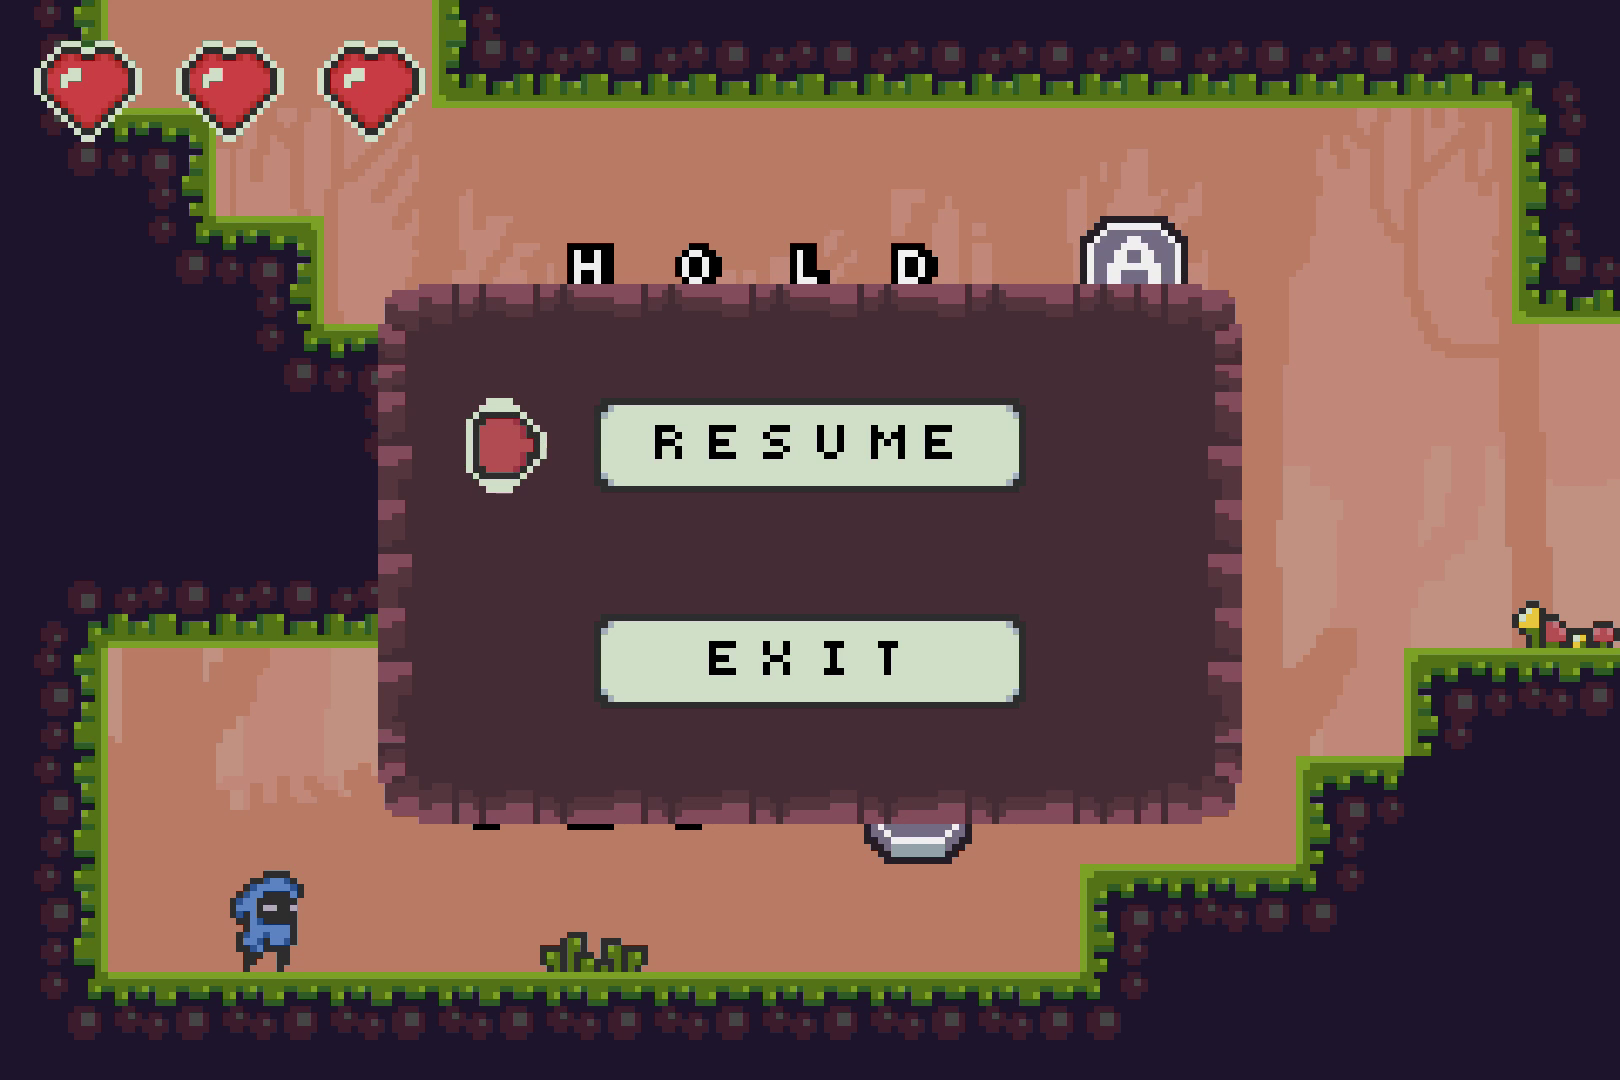
\includegraphics[height=6cm]{capitulos/apendice/ingame_menu.png}
	\caption{Menú ingame.}\label{fig:ap_ingame_menu}
\end{figure}

\begin{figure}[h]
	\centering
	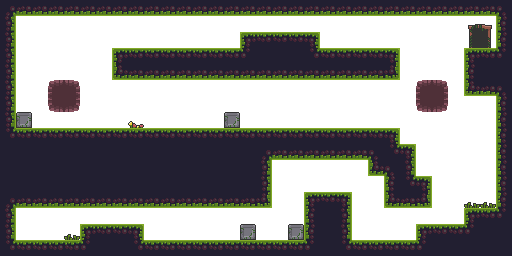
\includegraphics[height=7cm]{capitulos/apendice/level_2_0.png}
	\caption{Segundo nivel (1).}\label{fig:ap_lvl_2_0}
\end{figure}

\begin{figure}[h]
	\centering
	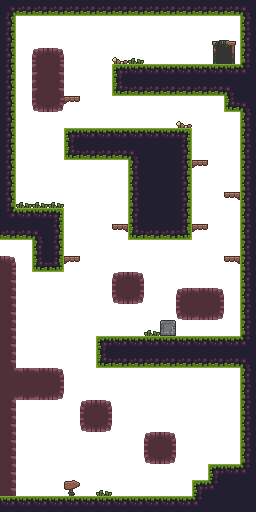
\includegraphics[height=14cm]{capitulos/apendice/level_2_1.png}
	\caption{Segundo nivel (2).}\label{fig:ap_lvl_2_1}
\end{figure}

\begin{figure}[h]
	\centering
	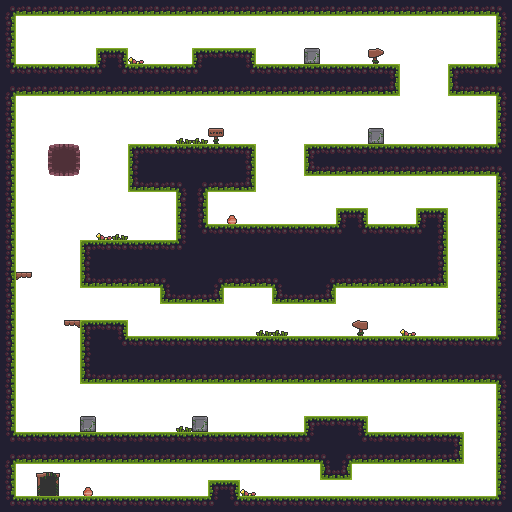
\includegraphics[height=14cm]{capitulos/apendice/level_3_0.png}
	\caption{Tercer nivel (1).}\label{fig:ap_lvl_3_0}
\end{figure}

\begin{figure}[h]
	\centering
	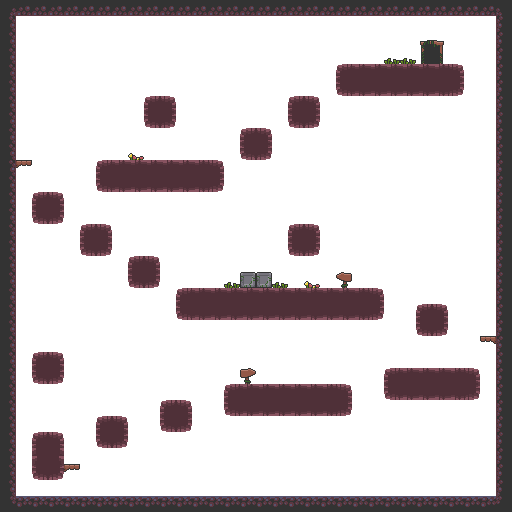
\includegraphics[height=14cm]{capitulos/apendice/level_3_1.png}
	\caption{Tercer nivel (2).}\label{fig:ap_lvl_3_1}
\end{figure}
\FloatBarrier{}

\section{Automatización mediante scripts de BASH}\label{ap:scripts}

\begin{lstlisting}[language=bash,breaklines=true,caption={Script (palettegen.sh) encargado de generar la paleta de colores para todas las imágenes proporcionadas.},label={lst:ap_palette}]

#!/bin/bash

if [ ! $# -ge 1 ]; then
	echo -e "usage:\t./script <images>"
	exit -1;
fi

TMP_FILE=.result.png

convert $@ -background none -append $TMP_FILE
superfamiconv palette -i $TMP_FILE -M gba -W 8 -H 8 --color-zero 000000 -d palette.bin -v
rm $TMP_FILE

\end{lstlisting}
\vspace{1cm}

\begin{lstlisting}[language=bash,breaklines=true,caption={Script (tilesgen.sh) encargado de generar un \textit{tileset} a partir de cada grupo de imágenes proporcionado. También hay que incluir la paleta generada anteriormente.},label={lst:ap_tiles}]

#!/bin/bash

if [ ! $# -ge 2 ]; then
	echo -e "usage:\t./script <images> <palette>"
	exit -1;
fi

TMP_FILE=.result.png

convert ${*%${!#}} -background none -append $TMP_FILE
superfamiconv tiles -i $TMP_FILE -p ${@:$#} -M gba -B 8 -W 8 -H 8 -d tiles.bin -v
rm $TMP_FILE

\end{lstlisting}
\vspace{1cm}

\begin{lstlisting}[language=bash,breaklines=true,caption={Script (mapgen.sh) encargado de generar un mapa a partir de un \textit{tileset}, paleta e imagen.},label={lst:ap_map}]

#!/bin/bash

if [ ! $# -eq 3 ]; then
	echo -e "usage:\t./script <image> <tiles> <palette>"
	exit -1;
fi

superfamiconv map -i $1 -t $2 -p $3 -M gba -B 8 -W 8 -H 8 -d map.bin -v

\end{lstlisting}
\newpage

\begin{lstlisting}[language=bash,breaklines=true,caption={Script encargado de procesar todas las imágenes utilizando palettegen.sh, tilesgen.sh y mapgen.sh.},label={lst:ap_map}]

#!/bin/bash

mkdir -p out

./include/palettegen.sh *.png

ls | grep -o "\w\+_" | sort -u | while read group; do
	./include/tilesgen.sh ${group}* palette.bin
	ls | grep "$group\w\+\.png" | while read file; do
		./include/mapgen.sh $file tiles.bin palette.bin
		name=`echo $file | sed 's/.png//g'`
		mv map.bin out/${name}_map.bin
	done
	mv tiles.bin out/${group}tiles.bin
done

mv palette.bin out/palette.bin

\end{lstlisting}

\section{Funciones de la BIOS}\label{ap:bios}

\begin{table}[h]
	\centering
	\begin{tabular}{| c | c |}
		\hline
		\textbf{Valor} & \textbf{Función}  \\ \hline
		0x00 & SoftReset \\ \hline
		0x01 & RegisterRamReset \\ \hline
		0x02 & Halt \\ \hline
		0x03 & Stop \\ \hline
		0x04 & IntrWait \\ \hline
		0x05 & VBlankIntrWait \\ \hline
		0x06 & Div \\ \hline
		0x07 & DivArm \\ \hline
		0x08 & Sqrt \\ \hline
		0x09 & ArcTan \\ \hline
		0x0A & ArcTan2 \\ \hline
		0x0B & CPUSet \\ \hline
		0x0C & CPUFastSet \\ \hline
		0x0D & BiosChecksum \\ \hline
		0x0E & BgAffineSet \\ \hline
		0x0F & ObjAffineSet \\ \hline
	\end{tabular}
	\caption{Funciones de la BIOS a utilizar con la instrucción \textit{swi} (1).}\label{tab:ap_bios_1}
\end{table}

\begin{table}[h]
	\centering
	\begin{tabular}{| c | c |}
		\hline
		\textbf{Valor} & \textbf{Función}  \\ \hline
		0x10 & BitUnPack \\ \hline
		0x11 & LZ77UnCompWRAM \\ \hline
		0x12 & LZ77UnCompVRAM \\ \hline
		0x13 & HuffUnComp \\ \hline
		0x14 & RLUnCompWRAM \\ \hline
		0x15 & RLUnCompVRAM \\ \hline
		0x16 & Diff8bitUnFilterWRAM \\ \hline
		0x17 & Diff8bitUnFilterVRAM \\ \hline
		0x18 & Diff16bitUnFilter \\ \hline
		0x19 & SoundBiasChange \\ \hline
		0x1A & SoundDriverInit \\ \hline
		0x1B & SoundDriverMode \\ \hline
		0x1C & SoundDriverMain \\ \hline
		0x1D & SoundDriverVSync \\ \hline
		0x1E & SoundChannelClear \\ \hline
		0x1F & MIDIKey2Freq \\ \hline
	\end{tabular}
	\caption{Funciones de la BIOS a utilizar con la instrucción \textit{swi} (2).}\label{tab:ap_bios_2}
\end{table}

\begin{table}[h]
	\centering
	\begin{tabular}{| c | c |}
		\hline
		\textbf{Valor} & \textbf{Función}  \\ \hline
		0x20 & MusicPlayerOpen \\ \hline
		0x21 & MusicPlayerStart \\ \hline
		0x22 & MusicPlayerStop \\ \hline
		0x23 & MusicPlayerContinue \\ \hline
		0x24 & MusicPlayerFadeOut \\ \hline
		0x25 & MultiBoot \\ \hline
		0x26 & HardReset \\ \hline
		0x27 & CustomHalt \\ \hline
		0x28 & SoundDriverVSyncOff \\ \hline
		0x29 & SoundDriverVSyncOn \\ \hline
		0x2A & GetJumpList \\ \hline
	\end{tabular}
	\caption{Funciones de la BIOS a utilizar con la instrucción \textit{swi} (3).}\label{tab:ap_bios_3}
\end{table}
\FloatBarrier{}

